

\begin{table*}[ht]
\centering
\small
\renewcommand{\arraystretch}{0.95}
\renewcommand\tabcolsep{4pt}
\begin{tabular}{cc|c|c|c|c|ccc}
\hline 
\multicolumn{2}{c|}{Dataset} & Model & Venue & Base & Method & mAP$\uparrow$ & Rank-1$\uparrow$ & $\text{ID}^2$$\downarrow$ \\ \hline
% \multicolumn{2}{c|}{} & & & & ori & 3.34 & 11.4 & 0.5135 \\ \cline{6-9} 
% \multicolumn{2}{c|}{} & \multirow{-2}{*}{TransReID\cite{he2021transreid}(w/o training)} & & & +ours & 52.81\scriptsize{(+49.47)} & 78.92\scriptsize{(+67.52)} & 0.2158 \\ \cline{3-3} \cline{6-9} 
\multicolumn{2}{c|}{} & & & & official & 79.88 & 91.48 & 0.2193 \\ \cline{6-9} 
\multicolumn{2}{c|}{} & \multirow{-2}{*}{TransReID\cite{he2021transreid}(w/o camid)} & & & +ours & 90.39\scriptsize{(+10.51)} & 94.74\scriptsize{(+3.26)} & 0.1357 \\ \cline{3-3} \cline{6-9} 
\multicolumn{2}{c|}{} & & & & official & 89 & 95.1 & 0.2759 \\ \cline{6-9} 
\multicolumn{2}{c|}{} & \multirow{-2}{*}{TransReID\cite{he2021transreid}(w/ camid)} & \multirow{-4}{*}{ICCV21} & \multirow{-4}{*}{ViT} & +ours & 93.01\scriptsize{(+4.01)} & 95.52\scriptsize{(+0.42)} & 0.1967 \\ \cline{3-9} 
\multicolumn{2}{c|}{} & & & & official & 89.7 & 95.4 & 0.0993 \\ \cline{6-9} 
\multicolumn{2}{c|}{} & & & \multirow{-2}{*}{ViT} & +ours & 94\scriptsize{(+4.3)} & 96.4\scriptsize{(+1.0)} & 0.0624 \\ \cline{5-9} 
\multicolumn{2}{c|}{} & & & & official & 89.8 & 95.7 & 0.0877 \\ \cline{6-9} 
\multicolumn{2}{c|}{\multirow{-8}{*}{Market1501}} & \multirow{-4}{*}{CLIP-ReID\cite{li2023clip}} & \multirow{-4}{*}{AAAI23} & \multirow{-2}{*}{CNN} & \cellcolor{gray!20}+ours & \cellcolor{gray!20}94.9\scriptsize{(+5.1)} & \cellcolor{gray!20}97.3\scriptsize{(+1.6)} & \cellcolor{gray!20}0.053 \\ \hline
\multicolumn{2}{c|}{} & & & & official & 79.05 & 85.4 & 0.3124 \\ \cline{6-9} 
\multicolumn{2}{c|}{} & \multirow{-2}{*}{KPR\cite{somers2025keypoint}} & \multirow{-2}{*}{ECCV24} & \multirow{-2}{*}{ViT} & \cellcolor{gray!20}+ours & \cellcolor{gray!20}89.34\scriptsize{(+10.29)} & \cellcolor{gray!20}91\scriptsize{(+5.6)} & \cellcolor{gray!20}0.1434 \\ \cline{3-9} 
\multicolumn{2}{c|}{} & & & & official & 70.41 & 77.2 & 0.377 \\ \cline{6-9} 
\multicolumn{2}{c|}{\multirow{-4}{*}{Occluded-ReID}} & \multirow{-2}{*}{BPBReID\cite{somers2023body}} & \multirow{-2}{*}{WACV23} & \multirow{-2}{*}{ViT} & +ours & 86.05\scriptsize{(+15.64)} & 89.1\scriptsize{(+11.9)} & 0.1504 \\ \hline
\multicolumn{1}{c|}{} & & & & & official & 71.81 & 75.29 & 0.4817 \\ \cline{6-9} 
\multicolumn{1}{c|}{} & \multirow{-2}{*}{All} & & & & \cellcolor{gray!20}+ours & \cellcolor{gray!20}76.44\scriptsize{(+4.63)} & \cellcolor{gray!20}79.33\scriptsize{(+4.04)} & \cellcolor{gray!20}0.4072 \\ \cline{2-2} \cline{6-9} 
\multicolumn{1}{c|}{} & & & & & official & 84.6 & 81.59 & 0.4424 \\ \cline{6-9} 
\multicolumn{1}{c|}{} & \multirow{-2}{*}{Indoor} & \multirow{-4}{*}{SAAI\cite{fang2023visible}} & \multirow{-4}{*}{ICCV23} & \multirow{-4}{*}{CNN} & \cellcolor{gray!20}+ours & \cellcolor{gray!20}86.83\scriptsize{(+2.23)} & \cellcolor{gray!20}84.2\scriptsize{(+2.61)} & \cellcolor{gray!20}0.3694 \\ \cline{2-9} 
\multicolumn{1}{c|}{} & & & & & official & 66.13 & 67.7 & 0.4308 \\ \cline{6-9} 
\multicolumn{1}{c|}{} & \multirow{-2}{*}{All} & & & & +ours & 75.43\scriptsize{(+9.3)} & 74.81\scriptsize{(+7.11)} & 0.3133 \\ \cline{2-2} \cline{6-9} 
\multicolumn{1}{c|}{} & & & & & official & 77.81 & 72.95 & 0.4046 \\ \cline{6-9} 
\multicolumn{1}{c|}{\multirow{-8}{*}{SYSU-MM01}} & \multirow{-2}{*}{Indoor} & \multirow{-4}{*}{PMT\cite{lu2023learning}} & \multirow{-4}{*}{AAAI23} & \multirow{-4}{*}{ViT} & +ours & 84.29\scriptsize{(+6.48)} & 80.29\scriptsize{(+7.34)} & 0.2995 \\ \hline
\end{tabular}

\caption{Improvements with our method on different SOTA models with both ViT and CNN backbone on Market1501, SYSU-MM01, and Occluded-ReID datasets. The data under \colorbox{gray!20}{grey} is the new SOTA with our methods of that dataset.}
\label{tab:sota}
\end{table*}


\begin{table*}[ht]
\centering
\small
\renewcommand{\arraystretch}{1.0}
\renewcommand\tabcolsep{4pt}
\begin{minipage}{0.32\textwidth}
\centering
\begin{tabular}{c|ccc}
\hline
\textbf{Methods} & mAP$\uparrow$ & Rank-1$\uparrow$ & $\text{ID}^2$$\downarrow$ \\ \hline
Base & 79.88 & 91.48 & 0.2193 \\
+NFC & 83.92 & 91.83 & 0.1824 \\
+IPG & 88.02 & 94.77 & 0.1553 \\
\rowcolor{gray!20}
+NFC+IPG & 90.39 & 94.74 & 0.1357 \\
\hline
\end{tabular}
\caption{Ablation study on effects of feature centralization through Identity-Guided Pedestrian Generation (IPG) and Neighbor Feature Centralization (NFC).}
\label{tab:ablation_fe_pg}
\end{minipage}
\hfill
\begin{minipage}{0.32\textwidth}
\centering
\begin{tabular}{cc|cc}
\hline
$\text{Gallery}^\text{NFC}$ & $\text{Query}^\text{NFC}$  & mAP$\uparrow$ & Rank-1$\uparrow$ \\ \hline
 \ding{55} & \ding{55}   & 79.88&	91.48  \\
 \ding{51} & \ding{55}    & 81.70 & 92.04  \\
\ding{55} & \ding{51}    & 82.76 & 91.69  \\
\rowcolor{gray!20}
\ding{51} & \ding{51}    & 83.92 & 91.83 \\ 
\hline
\end{tabular}
\caption{Ablation study of Neighbor Feature Centralization (NFC) Algorithm on Market1501 dataset. We test on the gallery and query set respectively.}
\label{tab:as_fe}
\end{minipage}
\hfill
\begin{minipage}{0.32\textwidth}
\centering
\begin{tabular}{cc|cc}
\hline
% \multicolumn{2}{c|}{\textbf{Methods}}& \multicolumn{4}{c}{Metrics}  \\ \hline
$\text{Gallery}^\text{IPG}$ & $\text{Query}^\text{IPG}$  & mAP$\uparrow$ & Rank-1$\uparrow$ \\ \hline
\ding{55} & \ding{55}   & 79.88&	91.48  \\
% \ding{51} & \ding{55}    &  84.06 &91.48 \\
% \ding{55} & \ding{51}    & 81.01 &91.03  \\
% \rowcolor{gray!20}
% \ding{51} & \ding{51}    & 87.38& 94.63 \\ 
 \ding{51} & \ding{55}    & 84.65&	92.07  \\
\ding{55} & \ding{51}    & 82.18	&92.40  \\
\rowcolor{gray!20}
\ding{51} & \ding{51}    &88.02&	94.77 \\ 
\hline
\end{tabular}
\caption{Ablation study of Feature ID-Centralizing with Pedestrian Generation (IPG) on Market1501. We test on gallery and query set respectively.}
\label{tab:as_gen}
\end{minipage}
\end{table*}


\begin{table}
\small
    \centering
    \renewcommand{\arraystretch}{1}
    \renewcommand\tabcolsep{6pt}
    \begin{tabular}{c|ccccc}
        \hline
        \textbf{Method} & mAP$\uparrow$ & R1$\uparrow$ & R5$\uparrow$ & R10$\uparrow$ & $\text{ID}^2$$\downarrow$ \\ \hline
        w/o training & 3.34 & 11.4 & 21.88 & 28 & 0.5135 \\
        \rowcolor{gray!20}
        +IPG & 52.81 & 78.92 & 91.21 & 94.27 & 0.2158 \\
        \rowcolor{gray!20}
        +IPG+NFC & 57.27 & 82.39 & 90.17 & 92.81 & 0.1890 \\ \hline
    \end{tabular}
    \caption{ReID performance on Market1501 with only ImageNet pre-trained weights without ReID training. The distribution visualized in Fig.\ref{fig:noise_tsne}.}
    \label{tab:notraining}
\end{table}
\begin{figure}[H]
\centering
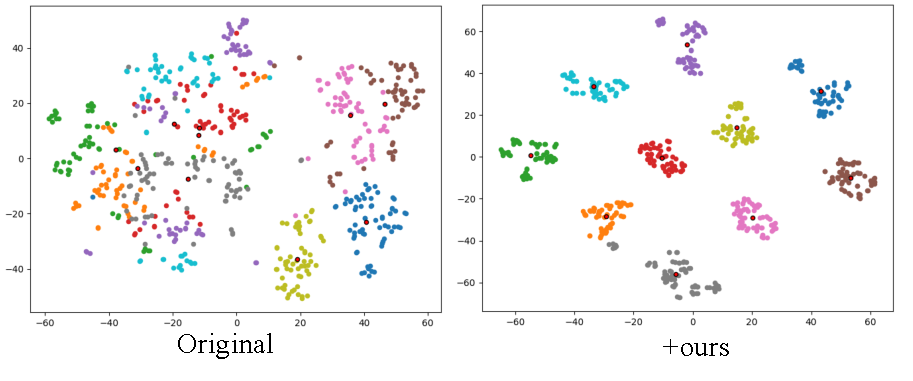
\includegraphics[width=0.95\linewidth]{figs/pdf/noise_tsne.pdf}
\caption{t-SNE visualization of 10 IDs feature distribution with and without our method on ImageNet pre-trained weights.}
\label{fig:noise_tsne}
\end{figure}


\section{Experiments}
\subsection{Implementation Details}

\textbf{Data Cleaning.}
Training an effective generative model requires high-quality data support. In current ReID (Person Re-Identification) datasets, there are many low-quality images, and removing them can help reduce interference to the model. In our experiments, we found two main issues that need to be addressed:\textbf{Extremely Low-quality Images}: The dataset contains images with such low resolution that even the human eye cannot recognize them as a "person". \textbf{Pose Estimation Failures}: The pose estimation model inevitably fails to detect pedestrian poses in some images.

Utilizing the feature distribution mentioned in Section\ref{Feature Distribution}, we can solve the issues and get the reference image set $S_i^{\text{ref}}$ and target image set $S^{\text{trg}}_i$ of identity $i$.
The cleansing process is detailed in \textbf{Supplementary}. 
\\
\textbf{Identity-guided Pedestrian Generation model details}
For the reference UNet and denoising UNet, we use the pretrained weights of Stable Diffusion v1.5\cite{rombach2022high}. The VAE encoder and decoder initialized with official weights\cite{kingma2013auto} and froze. For the ReID model, we use pre-trained TransReID\cite{he2021transreid} without cameras on Market1501 and freeze. 

The training data collected from training set of Market1501\cite{zheng2015scalable},  Mars\cite{zheng2016mars}, MSMT17\cite{wei2018person} and SYSU-MM01\cite{wu2017rgb}, with a total of 1946 different IDs. The model was trained for 80,000 iterations on one L20(48G) GPU with batch size of 4, which costs about 20 hours, and optimized by Adam\cite{kingma2014adam} with a learning rate of 1e-5 and weight decay of 0.01. All images are resized to 512×256. We applied random flip and random erasing\cite{zhong2020random} data augmentation only on reference images.

According to Section\ref{standard pose}, we selected 8 poses on the market1501 dataset as the representative poses. Each image in test set generates 8 images with these representative poses. The generation uses DDIM with 20 steps, classifier-free guidance with a scale of 3.5, and generator seed of 42.
\\
\textbf{ReID test settings}
Test models are loaded with official open-source pre-trained models for testing. In addition, considering the generated images do not have camera IDs, so for feature consistency, we test without camera IDs (e.g. TransReID). To validate the effectiveness of our proposed method, image flip (Section\ref{flip}) trick is \textbf{NOT} applied in our experiments. On Market1501, set \(\eta=2\), and \(k_1=k_2=2\). On Occluded REID, set \(\eta=1\), and \(k_1=k_2=1\). On SYSU-MM01, set \(\eta=1/4\), and \(k_1=k_2=2\). The parameters analysis detailed in \textbf{Supplementary}.



\subsection{Improvements on State-of-the-art Methods}
To verify the exceptional feature enhancement performance of our framework, we selected state-of-the-art models of three ReID tasks, divided into CNN and ViT-based models, to demonstrate that our theory can apply to any model and various ReID tasks. As shown in Table.\ref{tab:sota}, we achieved excellent enhancements on different models.

It is worth mentioning that we help models achieve new \textbf{SOTAs} without re-rank on 3 benchmarks:
\begin{itemize}
    \item[$\bullet$] \textbf{CNN-base CLIP-ReID on market1501: }
    
    \setlength{\parindent}{1em} mAP 94.9\%, Rank-1 97.3\%. 
    \item[$\bullet$] \textbf{KPR on Occluded-ReID: }

    \setlength{\parindent}{1em} mAP 89.34\%, Rank-1 91\%
    
    \item[$\bullet$] \textbf{SAAI on SYSU-MM01: }

    \setlength{\parindent}{1em} All-search mode: mAP 76.44\%, Rank-1 79.33\%
    
    \setlength{\parindent}{1em} Indoor-search mode: mAP 86.83\%, Rank-1 84.2\%
\end{itemize}



\subsection{ReID without Training}
TransReID loads a ViT pre-trained model on ImageNet for training on the ReID task. The pre-training method is based on contrastive learning strategies. According to the description in Section\ref{Feature Distribution}, training with contrastive loss helps to cluster features of same label samples. Images generated by our Pedestrian Generation model exhibit identity consistency, meaning they possess the attributes of the same label. Therefore, even if the features of an individual sample lack the pedestrian matching capability, as shown in the first row of Tab.\ref{tab:notraining}, its mAP and Rank-1 are only 3.34\% and 11.4\%. However, with our method, it improved 53.93\%/70.99\% to 57.27\%/82.39\%. Additionally, we visualized of 10 IDs' feature distributions using t-SNE as shown in Fig.\ref{fig:noise_tsne}.


\begin{figure}
\centering
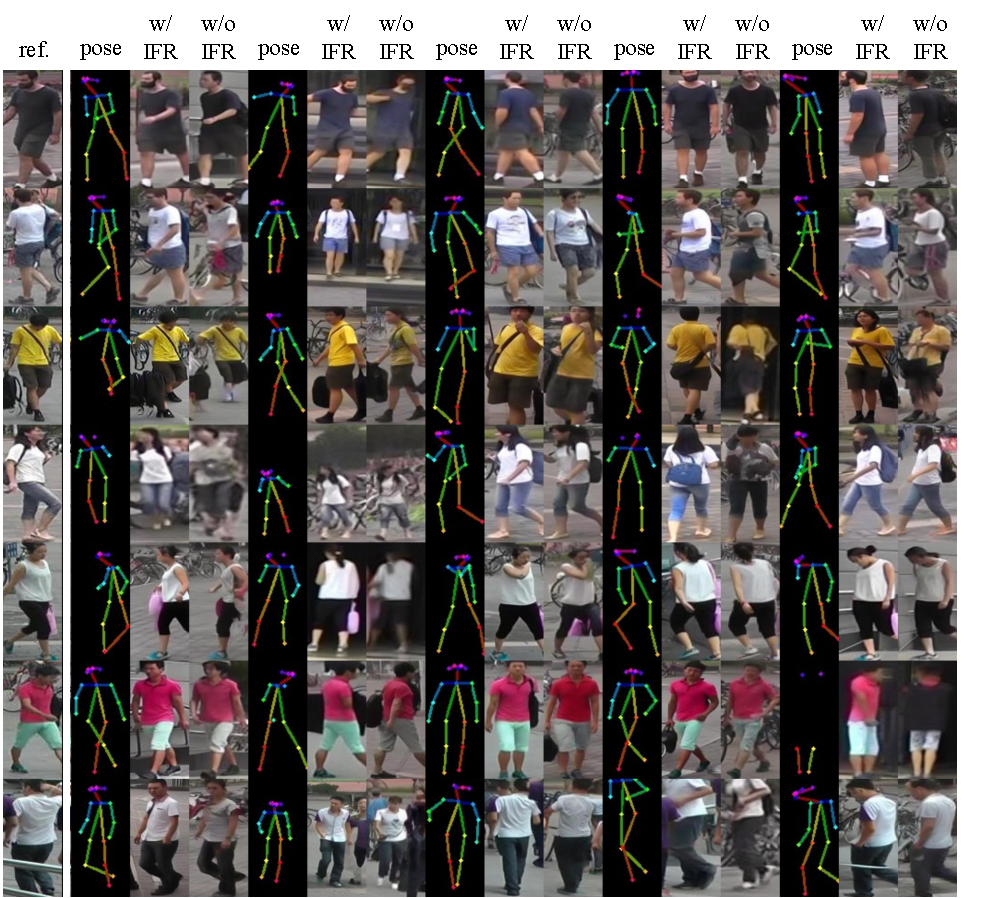
\includegraphics[width=0.95\linewidth]{figs/pdf/IFR.pdf}
\caption{The effects with and without the IFR module were visualized with five different poses randomly selected for each reference picture.}
\label{fig:IFR}
\end{figure}

\begin{table}
\small
    \centering
    \renewcommand{\arraystretch}{1}
    \renewcommand\tabcolsep{2pt}
    \begin{tabular}{c|ccc|ccc|ccc}
        \hline
        \multirow{2}{*}{\textbf{N}} & \multicolumn{3}{c|}{$\text{Gallery}^\text{IPG}$} & \multicolumn{3}{c|}{$\text{Query}^\text{IPG}$} & \multicolumn{3}{c}{$\text{Gallery}^\text{IPG}$+$\text{Query}^\text{IPG}$} \\ \cline{2-10}
          & mAP$\uparrow$ & R1$\uparrow$ & $\text{ID}^2$$\downarrow$ & mAP$\uparrow$ & R1$\uparrow$ & $\text{ID}^2$$\downarrow$ & mAP$\uparrow$ & R1$\uparrow$ & $\text{ID}^2$$\downarrow$ \\ \hline
        0 & 79.88 & 91.48 & 0.2313 & 79.88 & 91.48 & 0.1623 & 79.88 & 91.48 & 0.2193 \\
        1 & 80.96 & 90.97 & 0.2087 & 79.99 & 90.83 & 0.1363 & 82.13 & 92.01 & 0.1961 \\
        2 & 82.86 & 91.45 & 0.1904 & 81.17 & 92.04 & 0.1156 & 85.27 & 93.71 & 0.1773 \\
        3 & 83.42 & 91.75 & 0.1837 & 81.55 & 92.25 & 0.1077 & 86.16 & 94.21 & 0.1704 \\
        4 & 83.81 & 92.1  & 0.1795 & 81.76 & 92.34 & 0.1027 & 86.75 & 94.24 & 0.1661 \\
        5 & 84.07 & 91.83 & 0.1758 & 81.85 & 92.07 & 0.0984 & 87.23 & 94.71 & 0.1623 \\
        6 & 84.3  & 91.98 & 0.1730 & 81.96 & 92.52 & 0.0950 & 87.52 & 94.63 & 0.1593 \\
        7 & 84.49 & 91.86 & 0.1707 & 82.03 & 92.37 & 0.0922 & 87.76 & 94.60 & 0.1570 \\
        \rowcolor{gray!30}
        8 & 84.65 & 92.07 & 0.1691 & 82.18 & 92.40 & 0.0902 & 88.02 & 94.77 & 0.1553 \\ \hline
    \end{tabular}
    \caption{Performance Comparison by adding numbers of generated images for each image on gallery, query, and both}
    \label{tab:num}
\end{table}

\subsection{Abilation Study}
\textbf{Impact of the NFC and IPG.}
We conducted comprehensive ablation experiments on Neighbor Feature Centralization (NFC) and Feature ID-Centralizing through Identity-Guided Generation (IPG) methods. As shown in Table\ref{tab:ablation_fe_pg},\ref{tab:as_fe},\ref{tab:as_gen}, which show great improvements.
\begin{figure*}
\centering
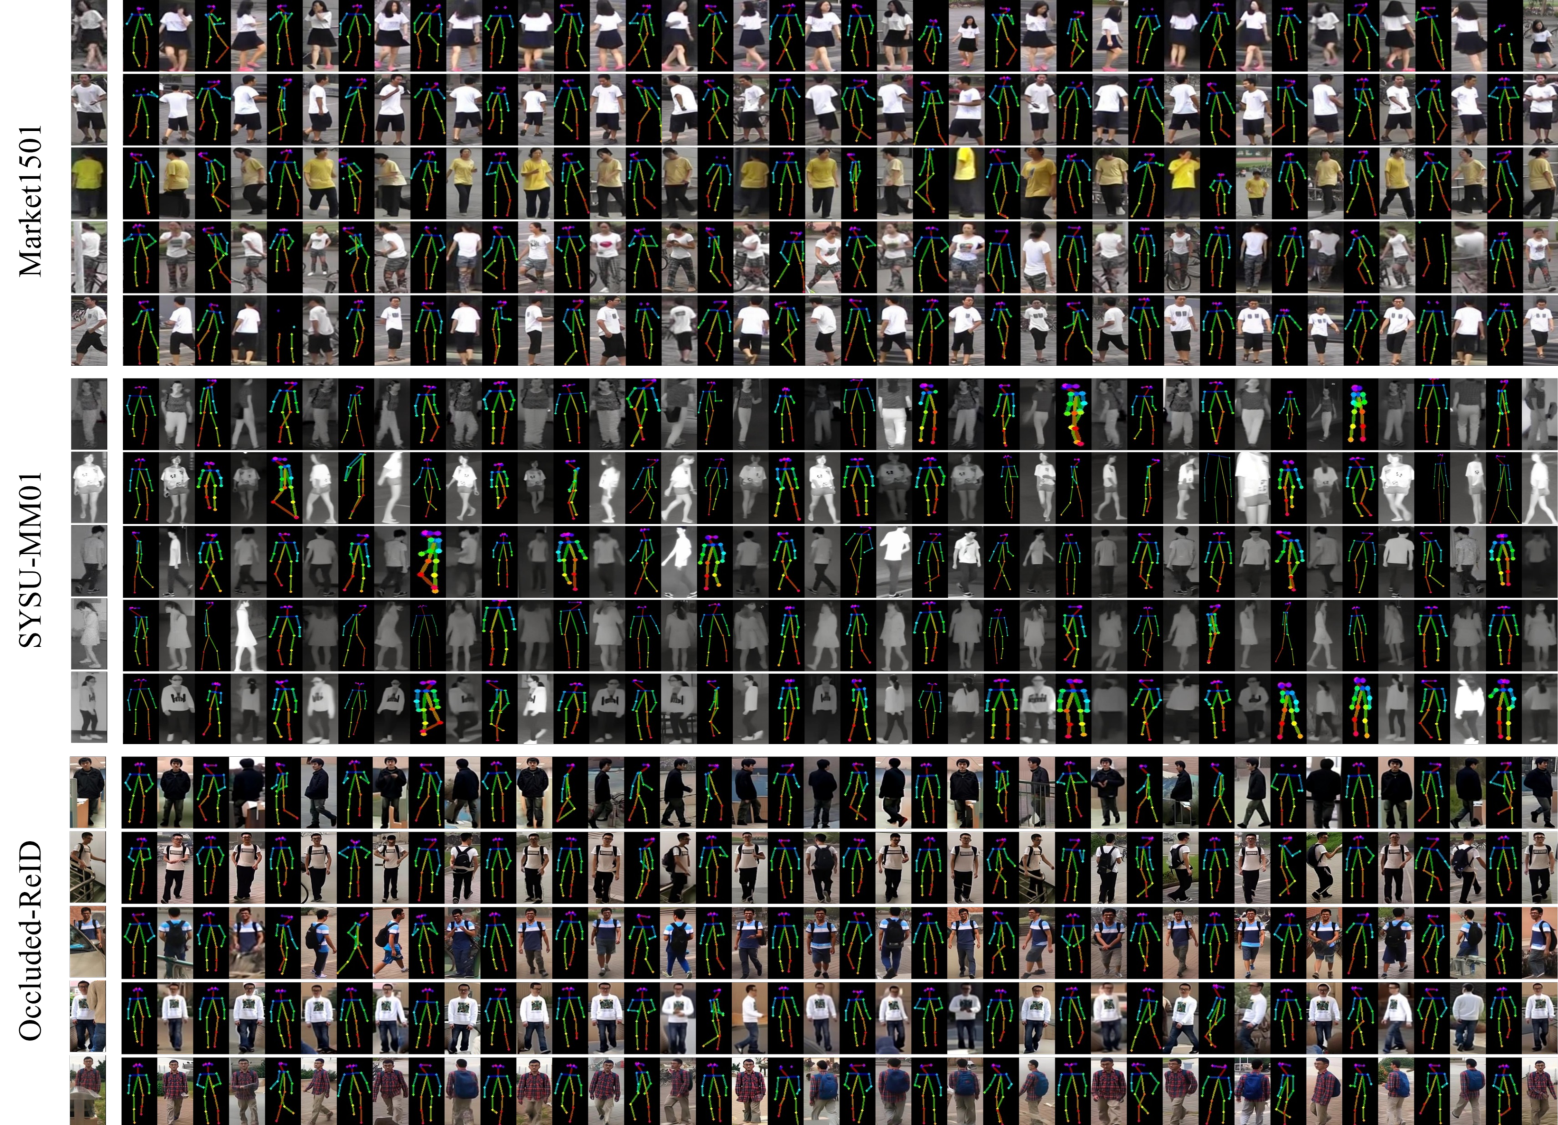
\includegraphics[width=\linewidth]{figs/pdf/random_sub_png.pdf}
\caption{Images generated with random poses. More randomly generated images can be found in Supplementary.}
\label{fig:randompose}
\end{figure*}
\\
\textbf{Effect of Feature Re-Distribute Module.}
We randomly selected 7 images from the Market1501 dataset, choosing 5 different poses for each image. We visualized the results both with and without Identity Feature Redistribute (IFR) Module. As shown in Fig.\ref{fig:IFR}, the impact of ID features on the generated outcomes is evident.
\\
\textbf{Effect of numbers of generated images.}
We randomly selected different numbers of images generated from the 8 representative poses to verify the effect of feature enhancement. As shown in Tab.\ref{tab:num}, the experimental results align with the theory mentioned in Section\ref{Feature Distribution}: the more features of the same ID that are aggregated, the more the adjustment noise extracted from individual images is reduced, enhancing the ID representation capability and resulting in improved matching performance.



\subsection{Visualizations}

\textbf{Different people with the same poses across datasets.}
We are working on Market1501, SYSU-MM01, and
Occluded-ReID datasets to visualize the 8 representative poses with only one model and results are shown in Fig.\ref{fig:intro}.
\\
\textbf{Random people with random poses.} To demonstrate the advancement of our model, as shown in Fig.\ref{fig:randompose}, we randomly chose samples from the whole dataset, and each sample randomly chose poses, including some problematic poses, fully demonstrating the diversity of model. \textbf{More examples on three datasets are visualized in }\textbf{Supplementary}.


% \subsection{Analysis on quality coefficient $\eta$ of Generation Model}

% Fig.\ref{fig:eta} illustrates the effect of adjusting the coefficient $\eta$ on the performance of the ReID model. To evaluate this impact, we gradually increased the value of $\eta$ and observed the changes in model performance on the mAP and Rank-1 metrics. 

% As the value of $\eta$ increases, the performance of the ReID model improves, reaching an optimal point. At $\eta = 2$, both mAP and Rank-1 achieve their maximum values of 88.02\% and 94.77\%, respectively. However, further increasing $\eta$ beyond this point leads to a slight decline in performance. It is easy to find that using generated images to centralize features is effective. However, considering the quality of the generated image, direct adding, although also effective, may not always achieve the best results. Therefore adjusting $\eta$ according to the generation quality of the model in this dataset can better centralize the features.
% \begin{figure}
% \centering
% 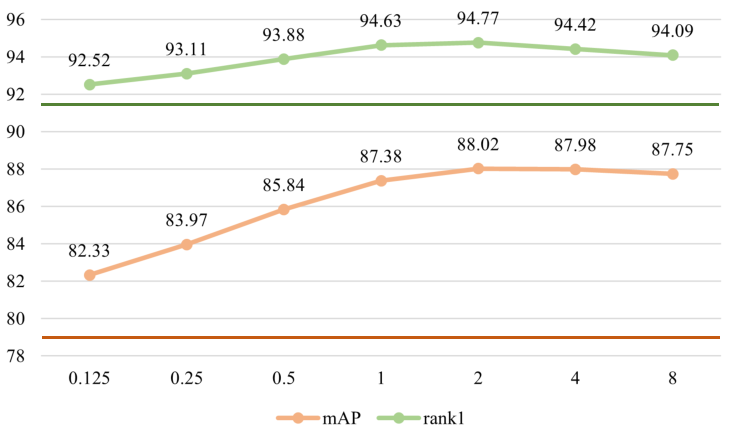
\includegraphics[width=0.9\linewidth]{figs/pdf/eta.pdf}
% \caption{Impact of the quality coefficient \( \eta \) with TransReID on Market1501. The dark color lines are the baseline.}
% \label{fig:eta}
% \end{figure}